In this chapter I will describe my implementation of a single-layer perceptron in Pharo. It will support multiclass classification (one or many neurons). Each neuron will be implemented as an object. The code of this project can be found is my NeuralNetwork repository on Smalltalkhub\footnote{http://smalltalkhub.com/\#!/~Oleks/NeuralNetwork}.

I will start by illustrating the design issues and different approaches to the implementation of every single part of this project. It will be quite long, so here is my final design:

\begin{figure}[H]
  \centering
  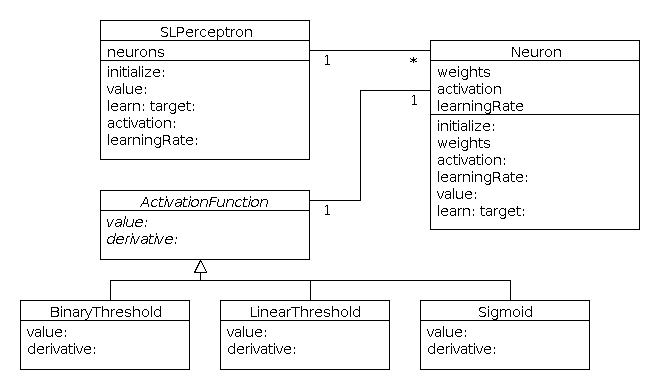
\includegraphics[width=0.9\linewidth]{slp}
  \caption{Object-oriented design of a single-layer perceptron}
  \label{fig:slp1}
\end{figure}

\section{What is a perceptron?}
First of all, we need to define a perceptron. It is the most basic form of an artificial neural network, still, most people fail to clearly define what it actually is.

For now I will refer to a perceptron as an artificial neural network that follows the perceptron learning procedure.

This definition implies some restrictions to what perceptrons are and what can they do.

\subsection{Restrictions of perceptrons}
\begin{itemize}
  \item They can only converge on a linearly-separable input (see XOR problem, Minski \& Pappet). But if the input is linearly-separable, the perceptron is guaranteed to converge on it, regardless of the initial weights and learning rate (see Perceptron Convergence Theorem, proven in 1962 by Block and Novikoff)
  \item Perceptrons (as defined above) can have only one layer of neurons. The thing is (week 3 of the Neural Networks for Machine Learning course by Geoffrey Hinton), the perceptron learning procedure can only be applied to a single layer of neurons. Neurons in hidden layers would need some sort of feedback in order to calculate their errors and update the weights. That’s why we need a different learning algorithm (e. g. backpropagation, which will be implemented on the next stage).
  \item Perceptrons can only learn online (one example at a time). That’s because the perceptron learning is based on adding (or subtracting) the input vector to the weights based on the error of a binary classifier (this error can be -1, 0, or 1).
\end{itemize}


\section{Design issues}
\subsection{How to represent weights?}
When it comes to the object-oriented implementation of neural networks, this is probably the most important question that has to be answered. Should weights belong to the neuron? If yes, should it be the sending or the receiving neuron? Or maybe they should belong to a layer? Or maybe to the whole network? Maybe we should even implement them as separate objects?

Being a feedforward network with only one layer, and therefore having no weights that connect two neurons, single-layer perceptron simplifies this problem. Basically, we have three options:
\begin{enumerate}
  \item Input weights of each neuron are stored as a vector inside that neuron.
  \item The matrix of all input weights is stored in the network.
  \item The weights are implemented as objects and connected to neurons.
\end{enumerate}

Second option is the most efficient (vector-matrix multiplication), but not very object-oriented. What is neuron in this implementation? Clearly, the network is just a matrix of weights + some learning rules. Should the neuron be an activation function with a learning rate? But then again, storing them in the network would be even more efficient. So basically, we don’t need a Neuron class. All we need is a matrix and several functions for manipulating it. That doesn’t sound object-oriented to me.

Third option in this case would be an over-engineering. It would just make the whole thing way more complicated. Implementing weights as objects would probably make some sense in a multi-layer neural network, where each weight is a connection between two neurons (we can think of inputs as of fake neurons). It connects two neurons, sends a signal between them and has a “strength” which can be updated. As a result, neurons would not know about other neurons. They would just receive, process, and emit the signals. I assume that such implementation would not be very fast, but it could be used for modeling purposes. I will write more about this idea in a post dedicated to multi-layer networks.

First option looks like most appropriate for single-layer perceptrons. And it’s very easy to implement, so I’ll stick to it.

\subsection{Activation functions}
There are two ways of representing activation functions in this project:

\begin{enumerate}
  \item Implement them as methods
  \item Implement them as classes
\end{enumerate}

The first approach will be faster and consume less memory. We create a base class Neuron with abstract methods activation and activationDerivative. Each subclass will be a special type of neuron, such as BinaryThresholdNeuron, SigmoidNeuron, that implements a corresponding activation function.

\begin{figure}[H]
  \centering
  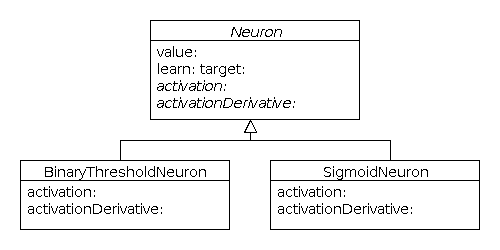
\includegraphics[width=0.8\linewidth]{activation1}
  \caption{Implementing activation functions as methods of specific subclasses on Neuron}
  \label{fig:activation1}
\end{figure}

Another way of implementing activations is to create a base class ActivationFunction with two abstract methods, value: and derivative:. This approach is more flexible, because if someone wants to use a new activation function, he will be able to implement it as a subclass, only defining what it is and what is its derivative. Then he will be able to pass an object of this class to an existing neuron. It doesn’t seem logical to reimplement the whole neuron every time we need to create a function.

\begin{figure}[H]
  \centering
  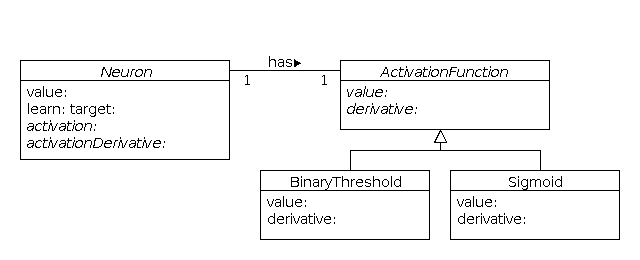
\includegraphics[width=0.9\linewidth]{activation2}
  \caption{Implementing activation functions as separate classes}
  \label{fig:activation2}
\end{figure}

So the real question can sound like this:
\textit{Are neurons defined by their activations? Does having a different activation means being a completely different type of neuron?}

\subsection{Shared or separate activation and learning rate?}
Both activation and learning rate can be either shared by all neurons of a perceptron or be stored separately in each neuron.The question is: do we need to have neurons with different activations and different learning rates?

Let’s assume that we don’t. Indeed, in most cases all neurons of a network (or a layer) share the same learning rate and have the same activation. If the network has many neurons (and most networks do), then we will be storing the same number just as many times. And if the activation function is implemented as a class, then we will be creating a separate instance of that class for each neuron.

However, if we wanted to parallelize the computations done by neurons, it would be better to have a separate learning rate and separate activation for each neuron (or each block of neurons). Otherwise they will just block each other trying to access the shared memory on every single step. And besides, the total memory occupied by this “heavy” neuron would still be rather small. I think, such neuron (or a group of them) would easily fit in the local memory of a single core of GPU.

But single-layer perceptrons do not usually perform heavy computations. They are more useful for the modeling purposes. That’s why we should probably take the “separate” approach and allow the user to build a network out of completely different neurons (like building blocks).

By the way, for multi-layer network the nice idea would be to share the same activation and learning rate inside one layer, but allow user to have completely different layers. In the end, he should be able to build some complicated network like the convolutional network on the picture. But that’s not the topic of this post.

\begin{figure}[H]
  \centering
  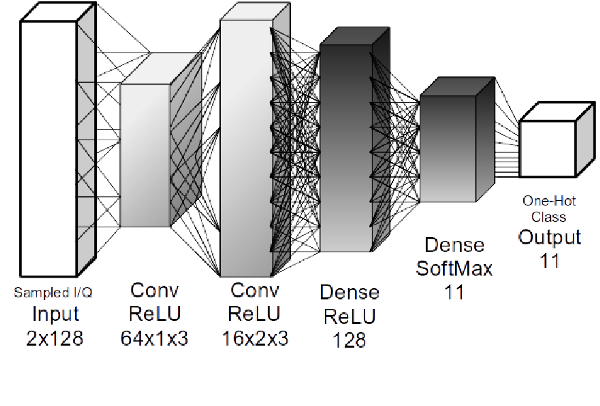
\includegraphics[width=0.8\linewidth]{conv}
  \caption{A convolutional neural network with four hidden layers}
  \label{fig:conv}
\end{figure}

\subsection{Data shuffling}
Online perceptrons are sensitive to the order in which training examples are received. Weight updates are made after each training example, that’s why the training vectors \#(\#(0 1) \#(1 1)) and \#(\#(1 1) \#(0 1)) will result in different weight vectors. Depending on the order of examples, the perceptron may need a different number of iterations to converge.

That’s why, to test the complexity of such learning, the perceptron has to be trained by examples randomly selected from a training set.


\section{Implementation}
Putting it all together, here is my design of a single-layer peceptron:

\begin{figure}[H]
  \centering
  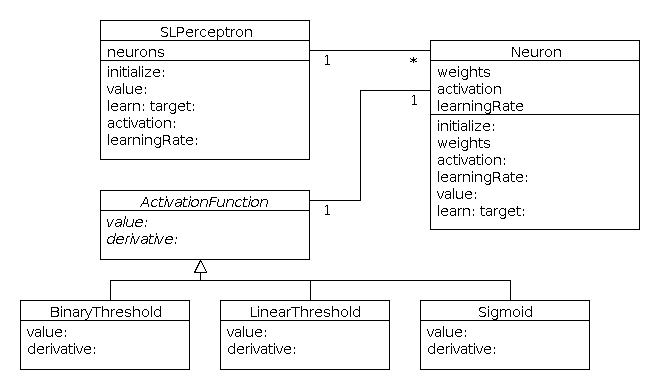
\includegraphics[width=0.9\linewidth]{slp}
  \caption{Object-oriented design of a single-layer perceptron}
  \label{fig:slp2}
\end{figure}

\subsection{Neuron class}
\begin{lstlisting}
Object subclass: #Neuron
   instanceVariableNames: 'weights activation learningRate'
   classVariableNames: ''
   package: 'NeuralNetwork'
\end{lstlisting}

The weights are initialized with random numbers in range [0, 1]. I’m not sure if this is a good range, but on simple examples it works just fine.

BinaryThreshold is a default activation function and the default learning rate is 0.1. These parameters can be changed using the accessors activation: and learningRate:.

\begin{lstlisting}
initialize: inputSize
   "Creates a weight vector and initializes it with random values. Assigns default values to activation and learning rate"

   activation := BinaryThreshold new.
   learningRate := 0.1.
 
   weights := DhbVector new: (inputSize + 1).
 
   1 to: (inputSize + 1) do: [ :i |
      weights at: i put: (1 / (10 atRandom))].
   ^ self
\end{lstlisting}

We will also need to prepend 1 as a bias unit to every input vector.

\begin{lstlisting}
prependBiasToInput: inputVector
   “this method prepends 1 to input vector for a bias unit”
 
   ^ (#(1), inputVector) asDhbVector.
\end{lstlisting}

According to “Numerical Methods” book, each function should implement the value: method. I want to emphasize that from the mathematical point of view neuron is a function.

Though the inner representation uses DhbVector, I want a user to write something like perceptron value: \#(1 0). instead of perceptron value: \#(1 0) asDhbVector.

\begin{lstlisting}
value: inputVector
   "Takes a vector of inputs and returns the output value"
 
   | inputDhbVector |
   inputDhbVector := self prependBiasToInput: inputVector.
   ^ activation value: (weights * inputDhbVector).
\end{lstlisting}

We need accessors for setting the learning rate an activation. I also added a simple accessor for weights for debugging purposes. All these accessors are trivial, so I will not put the code here.

And of course, the perceptron learning rule.

\begin{lstlisting}
learn: inputVector target: target
   "Applies the perceptron learning rule after looking at one training example"
 
   | input output error delta |
   output := self value: inputVector.
   error := target - output.
 
   input := self prependBiasToInput: inputVector.
  
   delta := learningRate * error * input * 
      (activation derivative: weights * input).
\end{lstlisting}
      
\subsection{SLPerceptron class}
Single-layer perceptron (according to my design) is a container of neurons. The only instance variable it has is the neurons array.

\begin{lstlisting}
Object subclass: #SLPerceptron
   instanceVariableNames: ‘neurons’
   classVariableNames: ‘’
   package: ‘NeuralNetwork’
\end{lstlisting}

To create an instance of SLPerceptron we need to specify the size of the input vector and the number of classes which equals to the number of neurons in our perceptron (multiclass classification).

\begin{lstlisting}
initialize: inputSize classes: outputSize
   “Creates an array of neurons”
   neurons := Array new: outputSize.
 
   1 to: outputSize do: [ :i |
      neurons at: i put: (Neuron new initialize: inputSize). ]
\end{lstlisting}

The output of a single-layer perceptron is a vector of scalar outputs from each neuron in the layer.

\begin{lstlisting}
value: input
   “Returns the vector of outputs from each neuron”
   | outputVector |
 
   outputVector := Array new: (neurons size).
 
   1 to: (neurons size) do: [ :i |
      outputVector at: i put: ((neurons at: i) value: input) ].
 
   ^ outputVector
\end{lstlisting}

If we ask SLPerceptron to learn, he will pass that request to all his neurons (basically, SLPerceptron is just a container of neurons that provides an interface for manipulating them).

\begin{lstlisting}
learn: input target: output
   "Trains the network (perceptron) on one (in case of online learning) or multiple (in case of batch learning) input/output pairs"

  1 to: (neurons size) do: [ :i |
     (neurons at: i) learn: input target: (output at: i) ].
\end{lstlisting}

     
\section{Testing}
I test my SLPerceptron with BinaryThreshold activation function on 4 linearly-separable logical functions: AND, OR, NAND, and NOR, and it converges on all of them.

Here is the test for AND function. Other 3 look exactly the same (only the expected output values are different).

\begin{lstlisting}
testANDConvergence
   "tests if perceptron is able to classify linearly-separable data"
   "AND function"

   | perceptron inputs outputs k |
   perceptron := SLPerceptron new initialize: 2 classes: 1.
   perceptron activation: (BinaryThreshold new).
 
   "logical AND function"
   inputs := #(#(0 0) #(0 1) #(1 0) #(1 1)).
   outputs := #(#(0) #(0) #(0) #(1)).
 
   1 to: 100 do: [ :i |
      k := 4 atRandom.
      perceptron learn: (inputs at: k) target: (outputs at: k) ].
 
   1 to: 4 do: [ :i |
      self assert: (perceptron value: (inputs at: i)) equals: (outputs at: i) ].
\end{lstlisting}

And this test (or rather a demonstration) shows that single-layer perceptron can not learn the XOR function (not linearly-separable).

\begin{lstlisting}
testXORDivergence
   "single-layer perceptron should not be uneble to classify data that is not linearly-separable"
   "XOR function"
   
   | perceptron inputs outputs k notEqual |
   perceptron := SLPerceptron new initialize: 2 classes: 1.
   perceptron activation: (BinaryThreshold new).
 
   "logical XOR function"
   inputs := #(#(0 0) #(0 1) #(1 0) #(1 1)).
   outputs := #(#(0) #(1) #(1) #(0)).
 
   1 to: 100 do: [ :i |
      k := 4 atRandom.
      perceptron learn: (inputs at: k) target: (outputs at: k) ].
 
   notEqual := false.
 
   1 to: 4 do: [ :i |
      notEqual := notEqual or:
         ((perceptron value: (inputs at: i)) ~= (outputs at: i)) ].
  
   self assert: notEqual.
\end{lstlisting}

I was also trying to test the Sigmoid function, but that test failed. This means that either perceptrons (as defined at the beginning of this post) can not have sigmoid as their activation, or that I don’t have a good enough understanding of how to implement a perceptron with sigmoid.

